%\setchapterpreamble[u]{\margintoc}
	\chapter{Macchine di Turing}
	Nascono in risposta al problema di Hilbert, che si chiedeva se esiste un algoritmo per dimostrare teoremi. Non ci sono comunque funzioni non calcolabili con le macchine di Turing:
	$$f:\mathbb{N}\to\{0,1\}\,\,s^{|\mathbb{N}}|>\mathbb{N}$$
	Siamo interessati a studiare la calcolabilità (computabilità).
	Esiste un programma che calcola una certa funzione? Se non esiste, $f$ è indecidibile. Se sì, in quanto tempo è calcolabile (complessità computazionale), quante mosse e quante celle del nastro sono necessarie?\\
	vediamo due esempi:
	\begin{example}
		data una CFG $G=(V,T,P,S)$ stabilire se è ambigua. Questo problema è indecidibile, cioè non esiste nessun algoritmo che dia una risposta.
	\end{example}
	\begin{example}
		Problema "ciao mondo": dato un sorgente di un programma in C/Java/..., i primi undici caratteri
		stampati dal programma sono "ciao, mondo"?
		Consideriamo il seguente algoritmo, che prende in input un numero intero N e stampa "ciao mondo" sse $\exists x,y,z\in \mathbb{N}$ tali che $x^n+y^n=z^n$
	\end{example}
	quest'ultimo problema è indecidibile:
	\begin{proof}
		procediamo per assurdo.\\Supponiamo che esista un algoritmo che risolva il problema.
		Assumiamo che P sia corretto (e quindi compilabile) e che stampi solo stringhe sulla console:
		\begin{center}
		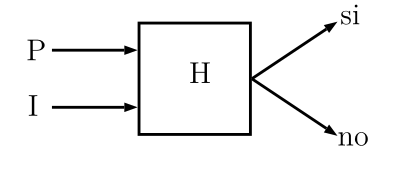
\includegraphics{2025-01-16_15-09.png}
			%\psscalebox{1.0 1.0} % Change this value to rescale the drawing.
			%{
			%	\begin{pspicture}(0,-0.965)(4.71,0.965)
			%		\psframe[linecolor=black, linewidth=0.04, dimen=outer](3.16,0.775)(1.56,-0.825)
			%		\psline[linecolor=black, linewidth=0.04, arrowsize=0.05291667cm 2.0,arrowlength=1.4,arrowinset=0.0]{->}(0.36,-0.425)(1.56,-0.425)
			%		\psline[linecolor=black, linewidth=0.04, arrowsize=0.05291667cm 2.0,arrowlength=1.4,arrowinset=0.0]{->}(0.36,0.375)(1.56,0.375)
			%		\psline[linecolor=black, linewidth=0.04, arrowsize=0.05291667cm 2.0,arrowlength=1.4,arrowinset=0.0]{->}(3.16,-0.025)(4.36,0.775)
			%		\psline[linecolor=black, linewidth=0.04, arrowsize=0.05291667cm 2.0,arrowlength=1.4,arrowinset=0.0]{->}(3.16,-0.025)(4.36,-0.825)
			%		\rput[bl](0.0,0.235){P}
			%		\rput[bl](0.02,-0.545){I}
			%		\rput[bl](2.28,-0.085){H}
			%		\rput[bl](4.4,0.735){si}
			%		\rput[bl](4.36,-0.965){no}
			%	\end{pspicture}
			%}
		\end{center}
		quindi:
		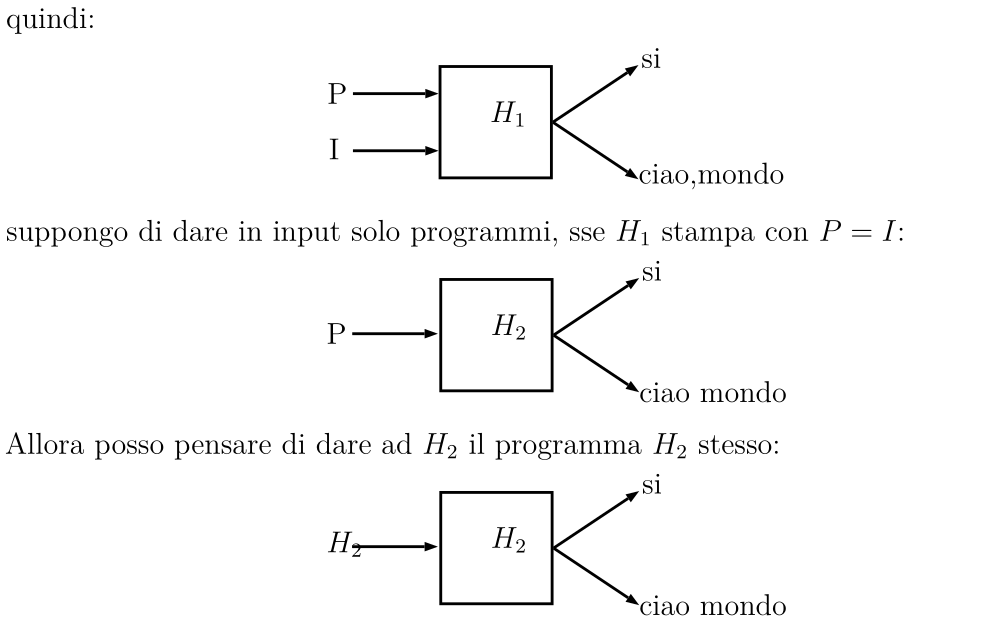
\includegraphics{2025-01-16_15-10.png}
		suppongo di dare in input solo programmi, sse $H_1$ stampa con $P=I$:
		Allora posso pensare di dare ad $H_2$ il programma $H_2$ stesso:
		Ma questo è assurdo: perché $H_2$ dice si quando in realtà stampa ciao mondo e viceversa, quindi
		non funziona. Ma allora in conclusione H non può esistere (perché i passaggi da H a $H_1$ e da $H_1$ a
		$H_2$ sono leciti) e quindi il problema non è decidibile.
	\end{proof}
	\section{Riduzioni}
	Supponiamo $P_2$ indicibile. Considerato un nuovo problema $P_2$, vorrei stabilire se anch'esso è
	indecidibile. Vorremmo quindi fare una "riduzione" da $P_1$ a $P_2$:
		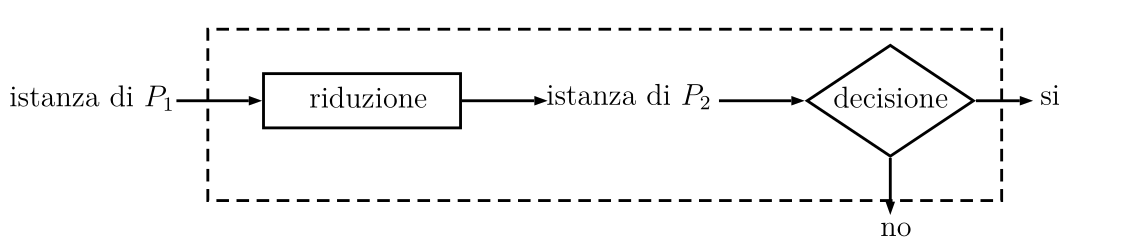
\includegraphics{2025-01-16_15-12.png}

	Supponiamo per assurdo che $P_2$ sia decidibile. Allora esiste l'algoritmo di decisione. Esistendo il
	processo di riduzione, allora l'intero rettangolo tratteggiato sarebbe un algoritmo di decisione per
$P_1$, assurdo perché $P_1$ è indecidibile per ipotesi.
	\begin{example}
		$P_2$ (Problema della chiamata): dato un programma $Q$, esso chiama il metodo $m()$?
		\\Dobbiamo quindi trovare un algoritmo di riduzione. Procediamo:
		\begin{itemize}
			\item rinominiamo tutte le istanze di $m$ in qualcosa d'altro
			\item aggiungiamo un metodo m che non verrà quindi mai chiamato
			\item modifichiamo questo programma in modo che salvi in un array i primi 11 caratteri che stampa a video
			\item modifichiamo questo programma in modo che se sfora gli 11 caratteri e controlla tali caratteri. Se sono esattamente "ciao mondo", chiama m
		\end{itemize}
		quindi anche questo problema è indecidibile
	\end{example}
	È importante che la riduzione sia fatta nel verso corretto. Se facessimo la riduzione da $P_2$ a $P_1$,
	staremmo mostrando che se $P_1$ è decidibile allora $P_2$ è decidibile. Ma sappiamo che $P_1$ è
	indecidibile, quindi non staremmo dimostrando niente.
	Nel caso contrario stiamo invece dicendo che se $P_2$ è decidibile allora $P_1$ è decidibile. Ma essendo
$P_1$ indecidibile, allora l'antecedente è falsa e quindi $P_2$ non può essere decidibile, quindi è
	indecidibile.\\
	Diamo ora la definizione formale della Macchina di Turing:
	\begin{definition}
		Si definisce MdT:
		$$M=(Q,\Sigma,\Gamma,\delta,q_0,B,F)$$
		con:
		\begin{itemize}
			\item $Q$ insieme finito non vuoto di stati
			\item $\Sigma$ insieme finito non vuoto di simboli di input
			\item $\Gamma$ insieme finito non vuoto di simboli sul nastro
			\item $\delta:Q\times\Gamma\to Q\times\Gamma\times\{L,R\}$
			\item $q_0\in Q$ stato iniziale
			\item $B\in\Gamma\backslash\Sigma$ simboli di blank
			\item $F\subseteq Q$ insieme di stati finali
		\end{itemize}
		inoltre si ha che:
		$$\Sigma\subseteq \Gamma\,\,\,e\,\,\,\Gamma\cap\Sigma\neq\emptyset$$
		quindi si ha per esempio questa rappresentazione, per l'input $x_1,...,x_n\in\Sigma^*$:
		\begin{center}
		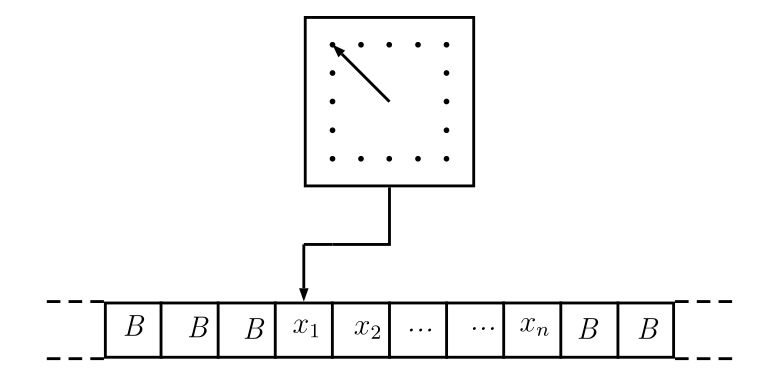
\includegraphics{2025-01-16_15-13.png}

			%\psscalebox{1.0 1.0} % Change this value to rescale the drawing.
			%{
			%	\begin{pspicture}(0,-2.41)(9.540835,2.41)
			%		\psframe[linecolor=black, linewidth=0.04, dimen=outer](6.0,2.41)(3.6,0.01)
			%		\psframe[linecolor=black, linewidth=0.04, dimen=outer](8.8,-1.59)(0.8,-2.39)
			%		\psline[linecolor=black, linewidth=0.04](4.8,0.01)(4.8,-0.79)(4.0,-0.79)
			%		\psline[linecolor=black, linewidth=0.04](1.6,-1.59)(1.6,-2.39)
			%		\psline[linecolor=black, linewidth=0.04](2.4,-1.59)(2.4,-2.39)
			%		\psline[linecolor=black, linewidth=0.04](3.2,-1.59)(3.2,-2.39)
			%		\psline[linecolor=black, linewidth=0.04](4.0,-1.59)(4.0,-2.39)
			%		\psline[linecolor=black, linewidth=0.04](4.8,-1.59)(4.8,-2.39)
			%		\psline[linecolor=black, linewidth=0.04](5.6,-1.59)(5.6,-2.39)
			%		\psline[linecolor=black, linewidth=0.04](6.4,-1.59)(6.4,-2.39)
			%		\psline[linecolor=black, linewidth=0.04](7.2,-1.59)(7.2,-2.39)
			%		\psline[linecolor=black, linewidth=0.04](8.0,-1.59)(8.0,-2.39)
			%		\psline[linecolor=black, linewidth=0.04, linestyle=dashed, dash=0.17638889cm 0.10583334cm](0.0,-1.59)(0.8,-1.59)
			%		\psline[linecolor=black, linewidth=0.04, linestyle=dashed, dash=0.17638889cm 0.10583334cm](0.0,-2.39)(0.8,-2.39)
			%		\psline[linecolor=black, linewidth=0.04, linestyle=dashed, dash=0.17638889cm 0.10583334cm](8.8,-1.59)(9.6,-1.59)
			%		\psline[linecolor=black, linewidth=0.04, linestyle=dashed, dash=0.17638889cm 0.10583334cm](8.8,-2.39)(9.6,-2.39)
			%		\psdots[linecolor=black, dotsize=0.08](4.0,2.01)
			%		\psdots[linecolor=black, dotsize=0.08](5.6,2.01)
			%		\psdots[linecolor=black, dotsize=0.08](5.6,1.21)
			%		\psdots[linecolor=black, dotsize=0.08](5.2,0.41)
			%		\psdots[linecolor=black, dotsize=0.08](4.4,0.41)
			%		\psdots[linecolor=black, dotsize=0.08](4.8,2.01)
			%		\psdots[linecolor=black, dotsize=0.08](4.0,1.21)
			%		\psdots[linecolor=black, dotsize=0.08](4.0,0.41)
			%		\psdots[linecolor=black, dotsize=0.08](5.6,0.41)
			%		\psdots[linecolor=black, dotsize=0.08](4.8,0.41)
			%		\psdots[linecolor=black, dotsize=0.08](4.4,2.01)
			%		\psdots[linecolor=black, dotsize=0.08](5.2,2.01)
			%		\psdots[linecolor=black, dotsize=0.08](5.6,1.61)
			%		\psdots[linecolor=black, dotsize=0.08](5.6,0.81)
			%		\psdots[linecolor=black, dotsize=0.08](4.0,1.61)
			%		\psdots[linecolor=black, dotsize=0.08](4.0,0.81)
			%		\psline[linecolor=black, linewidth=0.04, arrowsize=0.05291667cm 2.0,arrowlength=1.4,arrowinset=0.0]{->}(3.6,-0.79)(3.6,-1.59)
			%		\psline[linecolor=black, linewidth=0.04, arrowsize=0.05291667cm 2.0,arrowlength=1.4,arrowinset=0.0]{->}(4.8,1.21)(4.0,2.01)
			%		\psline[linecolor=black, linewidth=0.04](4.0,-0.79)(3.6,-0.79)
			%		\rput[bl](3.44,-2.09){$x_1$}
			%		\rput[bl](6.62,-2.07){$x_n$}
			%		\rput[bl](4.3,-2.11){$x_2$}
			%		\rput[bl](5.04,-2.01){...}
			%		\rput[bl](5.92,-1.99){...}
			%		\rput[bl](7.42,-2.11){B}
			%		\rput[bl](8.26,-2.11){B}
			%		\rput[bl](2.74,-2.11){B}
			%		\rput[bl](1.96,-2.09){B}
			%		\rput[bl](1.06,-2.07){B}
			%	\end{pspicture}
			%}

		\end{center}
	\end{definition}
	\newpage
	Questa era una definizione deterministica, passiamo ora ad una definizione \textit{istantanea}:
	\begin{definition}
		suppongo di avere lo stato $q$, il nastro $x_1,...,x_n$ con la testina $x_i$. SI ha:
		$$ID:\,\,x_1x_2,...qx_ix_{i+1}...x_n$$
		e suppongo $Q\cap\Gamma=\emptyset$ senza perdere generalità e uso la simbologia dei $\vdash$ introdotta coi PDA. \\
		Se $\delta(q,x_i)=(p,y,L)$ allora $\vdash\,\, x_1x_2...x_{i-2}px_{i-1}yx_{i+1}...x_n$.\\
		Si hanno dei casi particolari:
		\begin{itemize}
			\item se $i=1$ si ha $qx_1x_2...x_n\vdash pByx_2...x_n$
			\item se $i=n\,\,y=B$ si ha $qx_1x_2...qx_n\vdash x_1x_2...x_{n-2}px_{n-1}$
		\end{itemize}
		a destra abbiamo invece:
		Se $\delta(q,x_i)=(p,y,R)$ allora $\vdash\,\, x_1x_2...x_{i-1}Ypx_{i+1}...x_n$.\\
		Si hanno dei casi particolari:
		\begin{itemize}
			\item se $i=1$ si ha $q_1x_2...x_{n-1}\vdash ypB$
			\item se $i=n\,\,y=B$ si ha $qx_1x_2...qx_n\vdash px_2...x_n$
		\end{itemize}
	\end{definition}
	\begin{example}
		sia $L=\{0^n1^n|\,n\geq 1\}$ un CFL. vediamo una tabella per capire l'azione della macchina:
		\begin{center}
			\begin{tabular}{c|c|c|c|c|c|}
				      & 0           & 1           & x           & y           & B           \\
				\hline
				$q_0$ & $(q_1,x,R)$ & --          & --          & $(q_3,y,R)$ & --          \\
				$q_1$ & $(q_1,0,R)$ & $(q_2,y,L)$ & --          & $(q_1,y,R)$ & --          \\
				$q_2$ & $(q_2,0,L)$ & --          & $(q_0,x,R)$ & $(q_2,y,L)$ & --          \\
				$q_3$ & --          & --          & --          & $(q_2,y,L)$ & $(q_4,B,R)$ \\
				$q_4$ & --          & --          & --          & --          & --
			\end{tabular}
		\end{center}
		ovvero, per esempio:
		$$000111$$
		$$x00111$$
		$$x00y11$$
		$$xx0yy1$$
		$$xxxyyy$$
		\newpage
		ma la tabella non è comodissima, usiamo quindi i diagrammi di transizione:
		\begin{center}
			\begin{tikzpicture}[shorten >=1pt,node distance=3cm,on grid,auto]
				\node[state, initial,accepting] (q_0) {$q_0$};
				\node[state] (q_1) [right=of q_0] {$q_1$};
				\node[state] (q_2) [right =of q_1] {$q_2$};
				\node[state] (q_3) [below =of q_0] {$q_3$};
				\node[state] (q_4) [right =of q_3] {$q_4$};

				\path[->]
				(q_0) edge node [align=center] {$0/x\rightarrow$} (q_1)
				edge node [align=center] {$y/y\rightarrow$} (q_3)
				(q_1) edge node {$1/y\leftarrow$} (q_2)
				edge [loop above] node [align=center] {$y/y\rightarrow$\\$0/0\rightarrow$} ()
				(q_2) edge [bend left =40] node {$x/x\rightarrow$} (q_0)
				edge [loop above] node [align=center] {$y/y\leftarrow$\\$0/0\leftarrow$} ()
				(q_3) edge  node {$B/B\rightarrow$} (q_4)
				edge [loop below] node [align=center] {$y/y\rightarrow$} ()
				;
			\end{tikzpicture}
		\end{center}
		e per l'input 0010 si hanno i seguenti passi:
		$$q_0010\vdash xq_1010\vdash x0q_110\vdash xq_20y0\vdash  q_2x0y0$$
		$$\vdash xxq_2y0\vdash xxyq_10\vdash xxy0q_1B$$
	\end{example}
	definiamo quini il linguaggio accettato da una macchina di Turing:
	$$M=(Q,\Sigma,\Gamma,\delta,q_0,B,F)$$
	$$L(M)=\{w\in\Sigma^*|q_0w\stackrel{*}{\vdash}\alpha p\beta\,\,p\in F\,\,\alpha,\beta\in\Gamma^*\}$$
	La classe dei linguaggi accettati dalle MdT sono i ricorsivamente enumerabili (RE).
	Le MdT possono anche calcolare le funzioni:
	\begin{example}
		$$f(n,m)=m-n=max(m-n,0)=\begin{cases}
				m-n\,\,m\geq n \\
				0\,\,\,\,\,m<n
			\end{cases}$$
		quindi se l'input fosse $0^m10^n$ si avrebbe in output $0^{m-n}$
	\end{example}
	si ha che se la MdT accetta, allora si ferma e che se la MdT non accetta, allora non si può dire se si ferma oppure no. Se non si ferma: linguaggi ricorsivamente enumerabili. Se si ferma sempre, otteniamo una sottoclasse che sono i linguaggi ricorsivi. Inoltre il problema dell'arresto, \textbf{halting problem}, è indecidibile e quindi i linguaggi ricorsivamente enumerabili sono quindi semidecibili.\\
	Si possono avere delle estensioni della macchina di Turing:
	\begin{itemize}
		\item macchina non deterministica; anziché una sequenza di ID avremmo un albero. Non si aggiunge comunque potenza di calcolo, perché posso simulare una nondet con una det che esplora questo albero
		\item MdT multinastro
		      Hanno un numero finito di nastri. In una mossa guarda lo stato del controllo e il simbolo sotto ciascuna delle testine, si muove in un nuovo stato, scrive un nuovo simbolo per ogni nastro e si muove indipendentemente su ogni nastro:
		      \begin{center}
		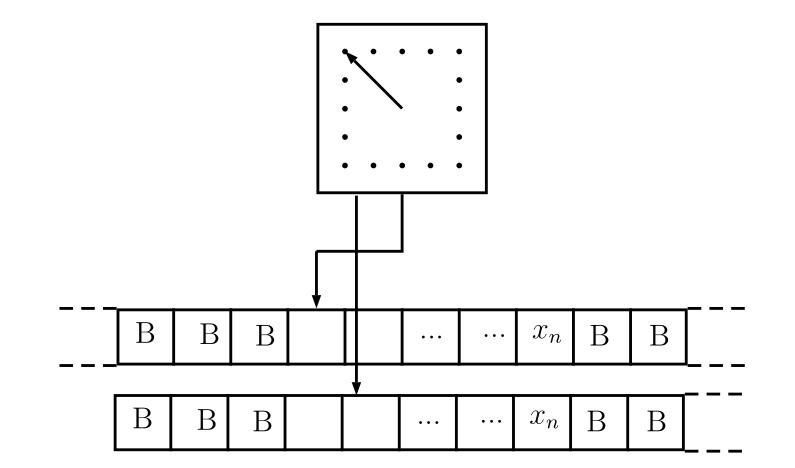
\includegraphics{2025-01-16_15-15.png}


			    %  \psscalebox{1.0 1.0} % Change this value to rescale the drawing.
			    %  {
				%      \begin{pspicture}(0,-3.01)(9.540835,3.01)
				%	      \psframe[linecolor=black, linewidth=0.04, dimen=outer](6.0,3.01)(3.6,0.61)
				%	      \psframe[linecolor=black, linewidth=0.04, dimen=outer](8.8,-0.99)(0.8,-1.79)
				%	      \psline[linecolor=black, linewidth=0.04](4.8,0.61)(4.8,-0.19)(4.0,-0.19)
				%	      \psline[linecolor=black, linewidth=0.04](1.6,-0.99)(1.6,-1.79)
				%	      \psline[linecolor=black, linewidth=0.04](2.4,-0.99)(2.4,-1.79)
				%	      \psline[linecolor=black, linewidth=0.04](3.2,-0.99)(3.2,-1.79)
				%	      \psline[linecolor=black, linewidth=0.04](4.0,-0.99)(4.0,-1.79)
				%	      \psline[linecolor=black, linewidth=0.04](4.8,-0.99)(4.8,-1.79)
				%	      \psline[linecolor=black, linewidth=0.04](5.6,-0.99)(5.6,-1.79)
				%	      \psline[linecolor=black, linewidth=0.04](6.4,-0.99)(6.4,-1.79)
				%	      \psline[linecolor=black, linewidth=0.04](7.2,-0.99)(7.2,-1.79)
				%	      \psline[linecolor=black, linewidth=0.04](8.0,-0.99)(8.0,-1.79)
				%%%%%%%%%%	      \psline[linecolor=black, linewidth=0.04, linestyle=dashed, dash=0.17638889cm 0.10583334cm](0.0,-0.99)(0.8,-0.99)
				%	      \psline[linecolor=black, linewidth=0.04, linestyle=dashed, dash=0.17638889cm 0.10583334cm](0.0,-1.79)(0.8,-1.79)
				%	      \psline[linecolor=black, linewidth=0.04, linestyle=dashed, dash=0.17638889cm 0.10583334cm](8.8,-0.99)(9.6,-0.99)
				%	      \psline[linecolor=black, linewidth=0.04, linestyle=dashed, dash=0.17638889cm 0.10583334cm](8.8,-1.79)(9.6,-1.79)
				%	      \psdots[linecolor=black, dotsize=0.08](4.0,2.61)
				%	      \psdots[linecolor=black, dotsize=0.08](5.6,2.61)
				%	      \psdots[linecolor=black, dotsize=0.08](5.6,1.81)
				%	      \psdots[linecolor=black, dotsize=0.08](5.2,1.01)
				%	      \psdots[linecolor=black, dotsize=0.08](4.4,1.01)
				%	      \psdots[linecolor=black, dotsize=0.08](4.8,2.61)
				%	      \psdots[linecolor=black, dotsize=0.08](4.0,1.81)
				%	      \psdots[linecolor=black, dotsize=0.08](4.0,1.01)
				%	      \psdots[linecolor=black, dotsize=0.08](5.6,1.01)
				%	      \psdots[linecolor=black, dotsize=0.08](4.8,1.01)
				%	      \psdots[linecolor=black, dotsize=0.08](4.4,2.61)
				%	      \psdots[linecolor=black, dotsize=0.08](5.2,2.61)
				%	      \psdots[linecolor=black, dotsize=0.08](5.6,2.21)
				%	      \psdots[linecolor=black, dotsize=0.08](5.6,1.41)
				%	      \psdots[linecolor=black, dotsize=0.08](4.0,2.21)
				%	      \psdots[linecolor=black, dotsize=0.08](4.0,1.41)
				%	      \psline[linecolor=black, linewidth=0.04, arrowsize=0.05291667cm 2.0,arrowlength=1.4,arrowinset=0.0]{->}(3.6,-0.19)(3.6,-0.99)
				%	      \psline[linecolor=black, linewidth=0.04, arrowsize=0.05291667cm 2.0,arrowlength=1.4,arrowinset=0.0]{->}(4.8,1.81)(4.0,2.61)
				%	      \psline[linecolor=black, linewidth=0.04](4.0,-0.19)(3.6,-0.19)
				%	      \rput[bl](6.62,-1.47){$x_n$}
				%	      \rput[bl](5.04,-1.41){...}
				%	      \rput[bl](5.92,-1.39){...}
				%	      \rput[bl](7.42,-1.51){B}
				%	      \rput[bl](8.26,-1.51){B}
				%	      \rput[bl](2.74,-1.51){B}
				%	      \rput[bl](1.96,-1.49){B}
				%	      \rput[bl](1.06,-1.47){B}
				%	      \psframe[linecolor=black, linewidth=0.04, dimen=outer](8.76,-2.19)(0.76,-2.99)
				%	      \psline[linecolor=black, linewidth=0.04](1.56,-2.19)(1.56,-2.99)
				%	      \psline[linecolor=black, linewidth=0.04](2.36,-2.19)(2.36,-2.99)
				%	      \psline[linecolor=black, linewidth=0.04](3.16,-2.19)(3.16,-2.99)
				%	      \psline[linecolor=black, linewidth=0.04](3.96,-2.19)(3.96,-2.99)
				%	      \psline[linecolor=black, linewidth=0.04](4.76,-2.19)(4.76,-2.99)
				%	      \psline[linecolor=black, linewidth=0.04](5.56,-2.19)(5.56,-2.99)
				%	      \psline[linecolor=black, linewidth=0.04](6.36,-2.19)(6.36,-2.99)
				%	      \psline[linecolor=black, linewidth=0.04](7.16,-2.19)(7.16,-2.99)
				%	      \psline[linecolor=black, linewidth=0.04](7.96,-2.19)(7.96,-2.99)
				%	      \psline[linecolor=black, linewidth=0.04, linestyle=dashed, dash=0.17638889cm 0.10583334cm](8.76,-2.19)(9.56,-2.19)
				%	      \psline[linecolor=black, linewidth=0.04, linestyle=dashed, dash=0.17638889cm 0.10583334cm](8.76,-2.99)(9.56,-2.99)
				%	      \psline[linecolor=black, linewidth=0.04, arrowsize=0.05291667cm 2.0,arrowlength=1.4,arrowinset=0.0]{->}(4.16,0.59)(4.16,-2.21)
				%	      \rput[bl](6.58,-2.67){$x_n$}
				%	      \rput[bl](5.0,-2.61){...}
				%	      \rput[bl](5.88,-2.59){...}
				%	      \rput[bl](7.38,-2.71){B}
				%	      \rput[bl](8.22,-2.71){B}
				%	      \rput[bl](2.7,-2.71){B}
				%	      \rput[bl](1.92,-2.69){B}
				%	      \rput[bl](1.02,-2.67){B}
				%      \end{pspicture}
			    %  }

		      \end{center}
	\end{itemize}
	si ha il seguente teorema:
	\begin{theorem}
		ogni linguaggio accettato da una MdT multinastro è Ricorsivamente Enumerabile
	\end{theorem}
	Ora possiamo definire in maniera più precisa cosa si intendeva per simulazione di una macchina
	nondet: uso due nastri, il primo con l'input e il secondo gestito come una coda di ID da elaborare
	\begin{theorem}
		Se Mn è una NTM (Nondeterministic Turing Machine) allora esiste una DTM
		(Deterministic Turing Machine) tale che il linguaggio accettato dalla NTM è uguale a quello accettato
		dalla DTM
	\end{theorem}
	\section{Restrizioni delle macchine di Turing}
	Consideriamo una MdT con nastro semiinfinito (ovvero è infinito solo da un lato):
	\begin{center}
			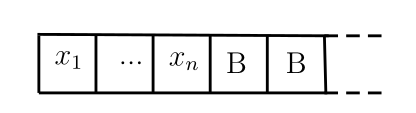
\includegraphics{2025-01-16_15-16.png}

		% \psscalebox{1.0 1.0} % Change this value to rescale the drawing.
		% {
		% 	\begin{pspicture}(0,-0.43)(4.7609334,0.43)
		% 		\psline[linecolor=black, linewidth=0.04](0.020098267,0.39)(0.020098267,-0.41)
		% 		\psline[linecolor=black, linewidth=0.04](0.8200983,0.39)(0.8200983,-0.41)
		% 		\psline[linecolor=black, linewidth=0.04](1.6200982,0.39)(1.6200982,-0.41)
		% 		\psline[linecolor=black, linewidth=0.04](2.4200983,0.39)(2.4200983,-0.41)
		% 		\psline[linecolor=black, linewidth=0.04](3.2200983,0.39)(3.2200983,-0.41)
		% 		\psline[linecolor=black, linewidth=0.04, linestyle=dashed, dash=0.17638889cm 0.10583334cm](4.020098,0.39)(4.8200984,0.39)
		% 		\psline[linecolor=black, linewidth=0.04, linestyle=dashed, dash=0.17638889cm 0.10583334cm](4.020098,-0.41)(4.8200984,-0.41)
		% 		\rput[bl](1.8400983,-0.09){$x_n$}
		% 		\rput[bl](0.24009827,-0.07){$x_1$}
		% 		\rput[bl](1.1400982,-0.01){...}
		% 		\rput[bl](2.6400983,-0.13){B}
		% 		\rput[bl](3.4800982,-0.13){B}
		% 		\psline[linecolor=black, linewidth=0.04](0.0,0.41)(4.080098,0.39)
		% 		\psline[linecolor=black, linewidth=0.04](0.020098267,-0.41)(4.040098,-0.41)(4.020098,0.39)
		% 	\end{pspicture}
		% }
	\end{center}
	si ha il seguente teorema:
	\begin{theorem}
		Ogni linguaggio accettato da una DTM M2 è anche accettato da una DTM M1 tale che:
		\begin{itemize}
			\item La testina di M1 non va mai a sinistra della posizione iniziale
			\item M1 non scrive mai un Blank:
			      $$B^{'}\not\in\Gamma \mbox{  e scrive }B^{'} \mbox{ al posto di } B$$
		\end{itemize}
	\end{theorem}
	Consideriamo ora una MdT tradizionale con il nastro:
			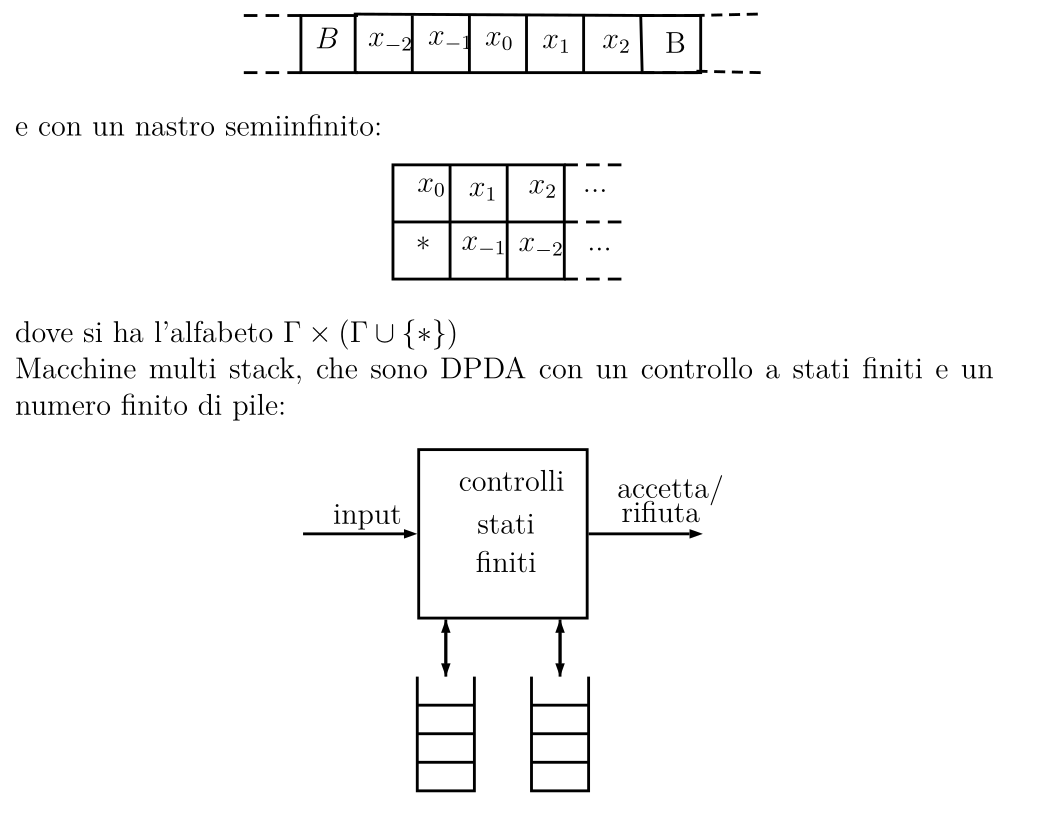
\includegraphics{2025-01-16_15-18.png}
	% \begin{center}

	% 	\psscalebox{1.0 1.0} % Change this value to rescale the drawing.
	% 	{
	% 		\begin{pspicture}(0,-0.43)(7.181278,0.43)
	% 			\psline[linecolor=black, linewidth=0.04](1.5008337,0.39)(1.5008337,-0.41)
	% 			\psline[linecolor=black, linewidth=0.04](2.3008337,0.39)(2.3008337,-0.41)
	% 			\psline[linecolor=black, linewidth=0.04](3.1008337,0.39)(3.1008337,-0.41)
	% 			\psline[linecolor=black, linewidth=0.04](3.9008338,0.39)(3.9008338,-0.41)
	% 			\psline[linecolor=black, linewidth=0.04](4.700834,0.39)(4.700834,-0.41)
	% 			\psline[linecolor=black, linewidth=0.04, linestyle=dashed, dash=0.17638889cm 0.10583334cm](5.5008335,0.39)(6.3008337,0.39)
	% 			\psline[linecolor=black, linewidth=0.04, linestyle=dashed, dash=0.17638889cm 0.10583334cm](5.5008335,-0.41)(6.3008337,-0.41)
	% 			\rput[bl](3.3208337,-0.09){$x_0$}
	% 			\rput[bl](1.6808337,-0.13){$x_{-2}$}
	% 			\rput[bl](2.5208337,-0.11){$x_{-1}$}
	% 			\rput[bl](4.120834,-0.13){$x_1$}
	% 			\rput[bl](4.9608335,-0.13){$x_2$}
	% 			\psline[linecolor=black, linewidth=0.04](1.4808338,0.41)(5.560834,0.39)
	% 			\psline[linecolor=black, linewidth=0.04](1.5008337,-0.41)(5.520834,-0.41)(5.5008335,0.39)
	% 			\psline[linecolor=black, linewidth=0.04](1.5408337,0.39)(0.74083376,0.39)(0.74083376,-0.41)(1.5408337,-0.41)
	% 			\psline[linecolor=black, linewidth=0.04, linestyle=dashed, dash=0.17638889cm 0.10583334cm](0.74083376,0.39)(-0.05916626,0.39)
	% 			\psline[linecolor=black, linewidth=0.04, linestyle=dashed, dash=0.17638889cm 0.10583334cm](0.74083376,-0.41)(-0.05916626,-0.41)
	% 			\rput[bl](0.94083375,-0.07){$B$}
	% 			\psline[linecolor=black, linewidth=0.04, linestyle=dashed, dash=0.17638889cm 0.10583334cm](6.2408338,0.39)(7.140834,0.41)
	% 			\psline[linecolor=black, linewidth=0.04, linestyle=dashed, dash=0.17638889cm 0.10583334cm](6.2808337,-0.39)(7.180834,-0.41)
	% 			\psline[linecolor=black, linewidth=0.04](5.540834,0.39)(6.3408337,0.39)(6.3408337,-0.41)(5.540834,-0.41)
	% 			\rput[bl](5.8408337,-0.13){B}
	% 		\end{pspicture}
	% 	}

	% \end{center}
	% e con un nastro semiinfinito:
	% \begin{center}

	% 	\psscalebox{1.0 1.0} % Change this value to rescale the drawing.
	% 	{
	% 		\begin{pspicture}(0,-0.82)(3.1608338,0.82)
	% 			\psline[linecolor=black, linewidth=0.04](0.02,-0.8)(2.42,-0.8)(2.42,0.8)(0.02,0.8)(0.02,-0.8)(0.82,-0.8)(0.82,0.8)(1.62,0.8)(1.62,-0.8)(2.42,-0.8)(2.42,0.0)(0.02,0.0)
	% 			\psline[linecolor=black, linewidth=0.04, linestyle=dashed, dash=0.17638889cm 0.10583334cm](2.42,0.8)(3.22,0.8)
	% 			\psline[linecolor=black, linewidth=0.04, linestyle=dashed, dash=0.17638889cm 0.10583334cm](2.42,0.0)(3.22,0.0)
	% 			\psline[linecolor=black, linewidth=0.04, linestyle=dashed, dash=0.17638889cm 0.10583334cm](2.42,-0.8)(3.22,-0.8)
	% 			\rput[bl](0.36,0.36){$x_0$}
	% 			\rput[bl](1.08,0.3){$x_1$}
	% 			\rput[bl](1.92,0.34){$x_2$}
	% 			\rput[bl](2.68,0.42){$...$}
	% 			\rput[bl](0.34,-0.52){*}
	% 			\rput[bl](0.98,-0.48){$x_{-1}$}
	% 			\rput[bl](1.78,-0.5){$x_{-2}$}
	% 			\rput[bl](2.74,-0.4){...}
	% 		\end{pspicture}
	% 	}

	% \end{center}
	% dove si ha l'alfabeto $\Gamma\times (\Gamma\cup\{*\})$\\
	% Macchine multi stack, che sono DPDA con un controllo a stati finiti e un numero finito di pile:
	% \begin{center}
	% 	\psscalebox{1.0 1.0} % Change this value to rescale the drawing.
	% 	{
	% 		\begin{pspicture}(0,-2.41)(5.64,2.41)
	% 			\psframe[linecolor=black, linewidth=0.04, dimen=outer](4.0,2.41)(1.6,0.01)
	% 			\psline[linecolor=black, linewidth=0.04, arrowsize=0.05291667cm 2.0,arrowlength=1.4,arrowinset=0.0]{->}(0.0,1.21)(1.6,1.21)
	% 			\psline[linecolor=black, linewidth=0.04, arrowsize=0.05291667cm 2.0,arrowlength=1.4,arrowinset=0.0]{->}(4.0,1.21)(5.6,1.21)
	% 			\psline[linecolor=black, linewidth=0.04, arrowsize=0.05291667cm 2.0,arrowlength=1.4,arrowinset=0.0]{->}(2.0,0.01)(2.0,-0.79)
	% 			\psline[linecolor=black, linewidth=0.04, arrowsize=0.05291667cm 2.0,arrowlength=1.4,arrowinset=0.0]{->}(2.0,-0.79)(2.0,0.01)
	% 			\psline[linecolor=black, linewidth=0.04, arrowsize=0.05291667cm 2.0,arrowlength=1.4,arrowinset=0.0]{->}(3.6,0.01)(3.6,-0.79)
	% 			\psline[linecolor=black, linewidth=0.04, arrowsize=0.05291667cm 2.0,arrowlength=1.4,arrowinset=0.0]{->}(3.6,-0.79)(3.6,0.01)
	% 			\psline[linecolor=black, linewidth=0.04](1.6,-0.79)(1.6,-2.39)(2.4,-2.39)(2.4,-0.79)(2.4,-1.19)(1.6,-1.19)(1.6,-1.59)(2.4,-1.59)(2.4,-1.99)(1.6,-1.99)(2.4,-1.99)
	% 			\psline[linecolor=black, linewidth=0.04](3.2,-0.79)(3.2,-2.39)(4.0,-2.39)(4.0,-0.79)(4.0,-1.19)(3.2,-1.19)(3.2,-1.59)(4.0,-1.59)(4.0,-1.99)(3.2,-1.99)(4.0,-1.99)
	% 			\rput[bl](0.42,1.27){input}
	% 			\rput[bl](4.4,1.61){accetta/}
	% 			\rput[bl](4.46,1.37){rifiuta}
	% 			\rput[bl](2.18,1.81){controlli}
	% 			\rput[bl](2.44,1.21){stati}
	% 			\rput[bl](2.42,0.67){finiti}
	% 		\end{pspicture}
	% 	}
	% \end{center}
	e si ha:
	$$\delta(q,a,x_1,x_2,...,x_k)=(p,\gamma_1,\gamma_2,...,\gamma_k)$$
	% \begin{example}
	% 	Legge l'input e lo spinge tutto sul primo stack (sfruttando un simbolo ausiliario di fine input):
	% 	\begin{center}
	% 		\psscalebox{1.0 1.0} % Change this value to rescale the drawing.
	% 		{
	% 			\begin{pspicture}(0,-2.98)(4.02,2.98)
	% 				\psframe[linecolor=black, linewidth=0.04, dimen=outer](4.0,2.98)(1.6,0.58)
	% 				\psline[linecolor=black, linewidth=0.04, arrowsize=0.05291667cm 2.0,arrowlength=1.4,arrowinset=0.0]{->}(0.0,1.78)(1.6,1.78)
	% 				\psline[linecolor=black, linewidth=0.04, arrowsize=0.05291667cm 2.0,arrowlength=1.4,arrowinset=0.0]{->}(2.0,0.58)(2.0,-0.22)
	% 				\psline[linecolor=black, linewidth=0.04, arrowsize=0.05291667cm 2.0,arrowlength=1.4,arrowinset=0.0]{->}(2.0,-0.22)(2.0,0.58)
	% 				\psline[linecolor=black, linewidth=0.04, arrowsize=0.05291667cm 2.0,arrowlength=1.4,arrowinset=0.0]{->}(3.6,0.58)(3.6,-0.22)
	% 				\psline[linecolor=black, linewidth=0.04, arrowsize=0.05291667cm 2.0,arrowlength=1.4,arrowinset=0.0]{->}(3.6,-0.22)(3.6,0.58)
	% 				\psline[linecolor=black, linewidth=0.04](1.6,-0.22)(1.6,-1.82)(2.4,-1.82)(2.4,-0.22)(2.4,-0.62)(1.6,-0.62)(1.6,-1.02)(2.4,-1.02)(2.4,-1.42)(1.6,-1.42)(2.4,-1.42)
	% 				\psline[linecolor=black, linewidth=0.04](3.2,-0.22)(3.2,-1.82)(4.0,-1.82)(4.0,-0.22)(4.0,-0.62)(3.2,-0.62)(3.2,-1.02)(4.0,-1.02)(4.0,-1.42)(3.2,-1.42)(4.0,-1.42)
	% 				\rput[bl](0.42,1.84){input}
	% 				\rput[bl](1.94,-0.44){a}
	% 				\rput[bl](1.92,-0.88){s}
	% 				\rput[bl](1.92,-1.28){a}
	% 				\rput[bl](1.92,-1.72){c}
	% 				\rput[bl](3.5,-0.44){c}
	% 				\rput[bl](3.5,-0.92){a}
	% 				\rput[bl](3.56,-1.3){s}
	% 				\rput[bl](3.56,-1.68){a}
	% 				\psline[linecolor=black, linewidth=0.04](1.6,-1.82)(1.6,-2.22)(2.4,-2.22)(2.4,-1.82)
	% 				\psline[linecolor=black, linewidth=0.04](3.2,-1.82)(3.2,-2.22)(4.0,-2.22)(4.0,-1.82)
	% 				\rput[bl](1.8,-2.14){$z_0$}
	% 				\rput[bl](3.44,-2.2){$z_0$}
	% 				\rput[bl](0.36,1.42){$casa\$$}
	% 				\psline[linecolor=black, linewidth=0.04](2.0,-2.22)(2.0,-2.62)
	% 				\psline[linecolor=black, linewidth=0.04](3.6,-2.62)(3.6,-2.22)
	% 				\psline[linecolor=black, linewidth=0.04](2.0,-2.62)(3.6,-2.62)
	% 				\rput[bl](2.26,-2.98){ribalto}
	% 				\psline[linecolor=black, linewidth=0.04, arrowsize=0.05291667cm 2.0,arrowlength=1.4,arrowinset=0.0]{->}(3.6,-2.62)(3.6,-2.22)
	% 			\end{pspicture}
	% 		}

	% 	\end{center}
	%\end{example}
	si ha un'ulteriore restrizione:
	Supponiamo che i simboli sulle pile possano essere solo $x$ o
$z_0$. Si riescono ancora a simulare le macchine di Turing
			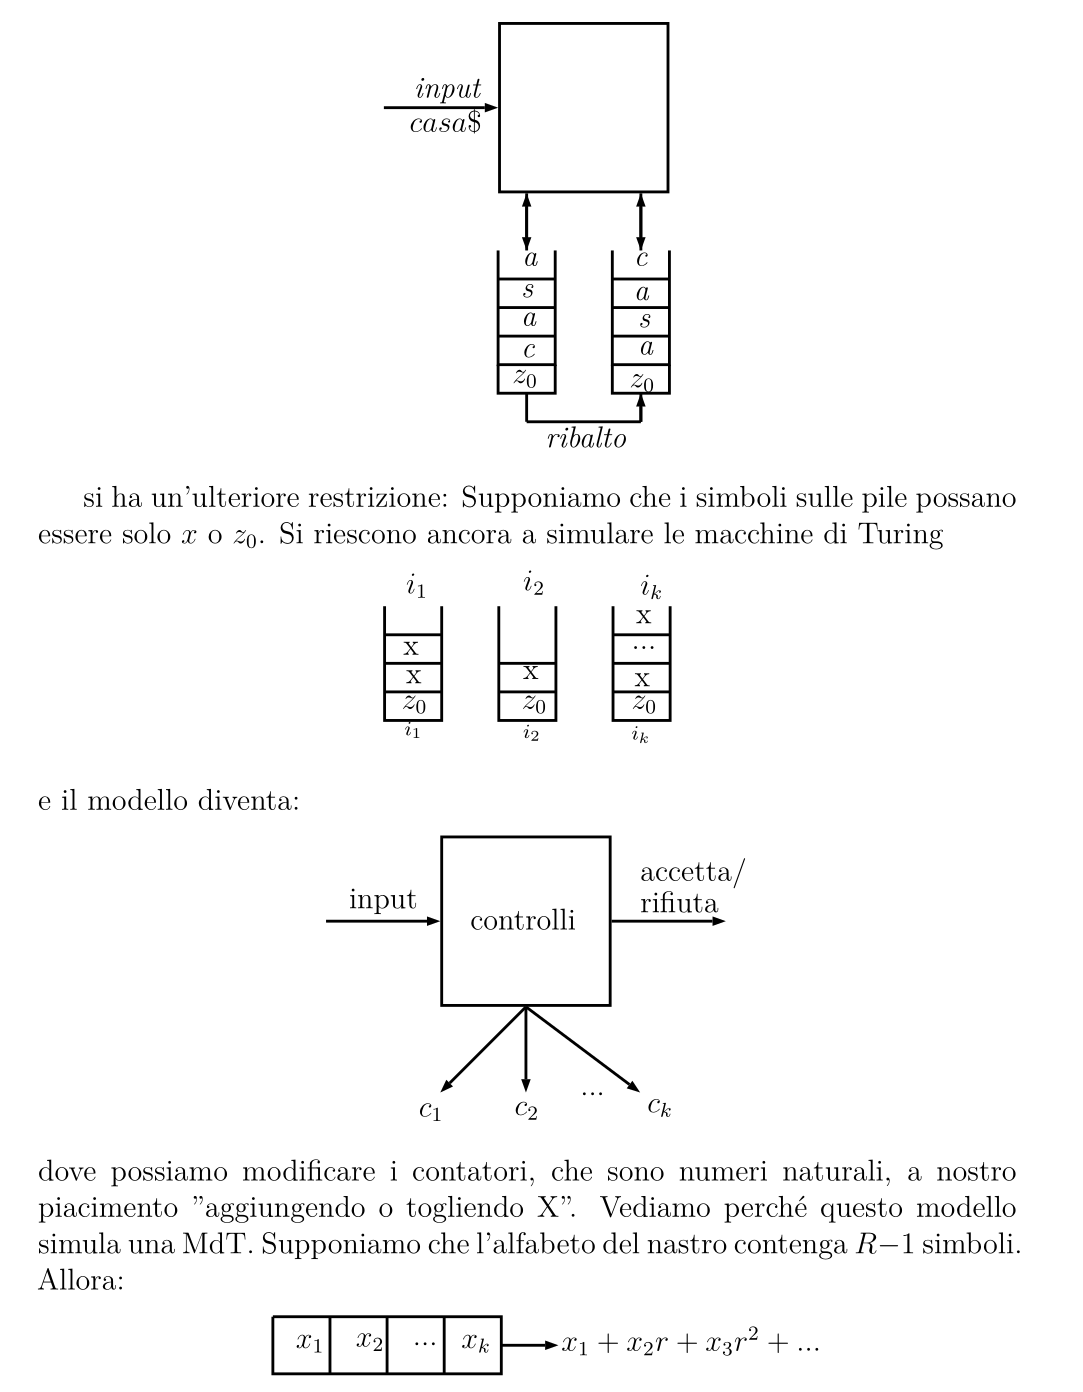
\includegraphics{2025-01-16_15-19.png}


% \begin{center}
% 		\psscalebox{1.0 1.0} % Change this value to rescale the drawing.
% 		{
% 			\begin{pspicture}(0,-1.23)(4.04,1.23)
% 				\psline[linecolor=black, linewidth=0.04](0.02,0.79)(0.02,-0.81)(0.82,-0.81)(0.82,0.79)(0.82,0.39)(0.02,0.39)
% 				\psline[linecolor=black, linewidth=0.04](0.02,-0.01)(0.82,-0.01)
% 				\psline[linecolor=black, linewidth=0.04](0.02,-0.41)(0.82,-0.41)
% 				\psline[linecolor=black, linewidth=0.04](1.62,0.79)(1.62,-0.81)(2.42,-0.81)(2.42,0.79)
% 				\psline[linecolor=black, linewidth=0.04](1.62,-0.01)(2.42,-0.01)
% 				\psline[linecolor=black, linewidth=0.04](1.62,-0.41)(2.42,-0.41)
% 				\psline[linecolor=black, linewidth=0.04](3.22,0.79)(3.22,-0.81)(4.02,-0.81)(4.02,0.79)(4.02,0.39)(3.22,0.39)
% 				\psline[linecolor=black, linewidth=0.04](3.22,-0.01)(4.02,-0.01)
% 				\psline[linecolor=black, linewidth=0.04](3.22,-0.41)(4.02,-0.41)
% 				\rput[bl](0.32,0.91){$i_1$}
% 				\rput[bl](0.28,0.11){x}
% 				\rput[bl](0.32,-0.29){x}
% 				\rput[bl](0.26,-0.71){$z_0$}
% 				\rput[bl](1.96,-0.23){x}
% 				\rput[bl](1.94,-0.71){$z_0$}
% 				\rput[bl](3.54,0.55){x}
% 				\rput[bl](3.48,0.19){...}
% 				\rput[bl](3.52,-0.33){x}
% 				\rput[bl](3.48,-0.71){$z_0$}
% 				\rput[bl](1.96,0.95){$i_2$}
% 				\rput[bl](3.6,0.89){$i_k$}
% 				\rput[bl](0.3,-1.17){$^{i_1}$}
% 				\rput[bl](1.96,-1.21){$^{i_2}$}
% 				\rput[bl](3.48,-1.23){$^{i_k}$}
% 			\end{pspicture}
% 		}
% 	\end{center}
% 	e il modello diventa:
% 	\begin{center}


% 		\psscalebox{1.0 1.0} % Change this value to rescale the drawing.
% 		{
% 			\begin{pspicture}(0,-2.0)(5.64,2.0)
% 				\psframe[linecolor=black, linewidth=0.04, dimen=outer](4.0,2.0)(1.6,-0.4)
% 				\psline[linecolor=black, linewidth=0.04, arrowsize=0.05291667cm 2.0,arrowlength=1.4,arrowinset=0.0]{->}(0.0,0.8)(1.6,0.8)
% 				\psline[linecolor=black, linewidth=0.04, arrowsize=0.05291667cm 2.0,arrowlength=1.4,arrowinset=0.0]{->}(4.0,0.8)(5.6,0.8)
% 				\psline[linecolor=black, linewidth=0.04, arrowsize=0.05291667cm 2.0,arrowlength=1.4,arrowinset=0.0]{->}(2.8,-0.4)(1.6,-1.6)
% 				\psline[linecolor=black, linewidth=0.04, arrowsize=0.05291667cm 2.0,arrowlength=1.4,arrowinset=0.0]{->}(2.8,-0.4)(2.8,-1.6)
% 				\psline[linecolor=black, linewidth=0.04, arrowsize=0.05291667cm 2.0,arrowlength=1.4,arrowinset=0.0]{->}(2.8,-0.4)(4.4,-1.6)
% 				\rput[bl](0.32,0.9){input}
% 				\rput[bl](2.02,0.68){controlli}
% 				\rput[bl](4.4,1.26){accetta/}
% 				\rput[bl](4.4,0.92){rifiuta}
% 				\rput[bl](1.3,-2.0){$c_1$}
% 				\rput[bl](2.64,-1.98){$c_2$}
% 				\rput[bl](3.56,-1.64){...}
% 				\rput[bl](4.5,-1.94){$c_k$}
% 			\end{pspicture}
% 		}

% 	\end{center}
% 	dove possiamo modificare i contatori, che sono numeri naturali, a nostro piacimento "aggiungendo
% 	o togliendo X". Vediamo perché questo modello simula una MdT.
% 	Supponiamo che l'alfabeto del nastro contenga $R-1$ simboli. Allora:
% 	\begin{center}

% 		\psscalebox{1.0 1.0} % Change this value to rescale the drawing.
% 		{
% 			\begin{pspicture}(0,-0.42)(7.17,0.42)
% 				\psline[linecolor=black, linewidth=0.04](0.02,0.4)(0.02,0.4)(3.22,0.4)(3.22,-0.4)(0.02,-0.4)(0.02,0.4)
% 				\psline[linecolor=black, linewidth=0.04](0.82,0.4)(0.82,-0.4)
% 				\psline[linecolor=black, linewidth=0.04](1.62,0.4)(1.62,-0.4)
% 				\psline[linecolor=black, linewidth=0.04](2.42,0.4)(2.42,-0.4)
% 				\psline[linecolor=black, linewidth=0.04, arrowsize=0.05291667cm 2.0,arrowlength=1.4,arrowinset=0.0]{->}(3.22,0.0)(4.02,0.0)
% 				\rput[bl](0.34,-0.1){$x_1$}
% 				\rput[bl](1.18,-0.08){$x_2$}
% 				\rput[bl](1.98,0.0){...}
% 				\rput[bl](2.66,-0.1){$x_k$}
% 				\rput[bl](4.06,-0.14){$x_1+x_2r+x_3r^2+...$}
% 			\end{pspicture}
% 		}

% 	\end{center}
	Così come codifico il nastro posso codificare una pila. Per togliere $x_1$ in cima alla pila devo dividere
	il numero per R e prendere il resto. Per aggiungere un nuovo simbolo, moltiplico per R e aggiungo il
	nuovo simbolo. Per modificare il simbolo, basta aggiungere la differenza tra il nuovo e la cima precedente. È immediato farlo con tre contatori (usandone uno di appoggio).
	Per fare tutto ciò bastano due contatori (e quindi due pile) dove nel primo è codificato come:
	$$2^{c_1}3^{c_2}5^{c_3}$$
	Per i linguaggi si ha quindi:
	\begin{itemize}
		\item linguaggi ricorsivi $\to$ decidibili e MdT si ferma sempre
		\item linguaggi ricorsivamente enumerabili $\to$ semidecidibili (ma comunque indecidibili) e MdT si ferma se accetta ma potrebbe non fermarsi
		\item linguaggi non ricorsivamente enumerabili $\to$ indecidibili e $\not\exists$ MdT
	\end{itemize}
	quindi, insiemisticamente:
	\begin{center}
			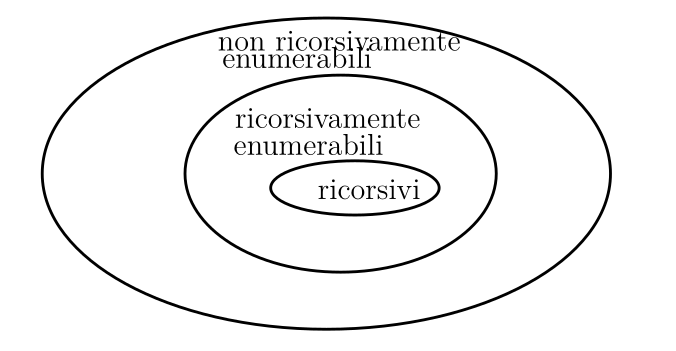
\includegraphics{2025-01-16_15-21.png}

		% \psscalebox{1.0 1.0} % Change this value to rescale the drawing.
		% {
		% 	\begin{pspicture}(0,-2.2)(8.0,2.2)
		% 		\psellipse[linecolor=black, linewidth=0.04, dimen=outer](4.0,0.0)(4.0,2.2)
		% 		\psellipse[linecolor=black, linewidth=0.04, dimen=outer](4.2,0.0)(2.2,1.4)
		% 		\psellipse[linecolor=black, linewidth=0.04, dimen=outer](4.4,-0.2)(1.2,0.4)
		% 		\rput[bl](2.48,1.72){non ricorsivamente }
		% 		\rput[bl](2.72,0.64){ricorsivamente }
		% 		\rput[bl](3.88,-0.36){ricorsivi}
		% 		\rput[bl](2.7,0.26){enumerabili}
		% 		\rput[bl](2.54,1.48){enumerabili}
		% 	\end{pspicture}
		% }

	\end{center}
	\begin{example}
		vediamo un linguaggio non ricorsivamente enumerabile.\\
		$w\in\{o,1\}^*$ biiezione tra stringhe e numeri:
		\begin{center}
			\begin{tabular}{c c c c c c c}
				$w_1$         & $w_2$ & $w_3$ & $w_4$ & $w_5$ & $w_6$ & ... \\
				1             & 2     & 3     & 4     & 5     & 6     & ... \\
				$\varepsilon$ & 0     & 1     & 00    & 01    & 10    & ..
			\end{tabular}
		\end{center}
		Consideriamo però le due stringe 00101 e 0101: se le leggessi come numeri binari sono entrambi
		5, quindi abbiamo perso la biiezione.
		Forziamo quindi l'interpretazione delle stringhe mettendoci davanti un 1.
		Codifichiamo anche una MdT in binario:
		$$M=(Q,\{0,1\},\Gamma,\delta,q_1,B,\{q_2\})$$
		$$Q=\{q_1,...,q_r\}$$
		$$\Gamma=\{x_1,...,x_s\}=\{0,1,B,...\}$$
		$$direzioni:\,\,L\to D_1\,\,R\to D_2$$
		$$\underbrace{\delta(q_i,x_j)=(q_k,x_1,D_m}_{0^i10^j10^k10^l10^m}$$
		$$Cod_111Cod_211Cod_3\\...=Cpd(\delta)$$
	\end{example}
	\begin{example}
		sia $M=(\{q_1,q_2,q_3\},\{o,1\}.\{0,1,B\},\delta,q_1,B,q_2)$ con:
		$$\overbrace{0}^{q_1}1\overbrace{00}^{x_2}1\overbrace{000}^{q_3}1\overbrace{0}^{x_1}1\overbrace{00}^{D_2}$$
		$$\delta(q_1,1)=(q_3,0,R)$$
		$$\delta(q_3,0)=(q_1,1,R)$$
		$$\delta(q_3,1)=(q_2,0,R)$$
		$$\delta(q_3,B)=(q_3,1,L)$$
		Quindi ora possiamo dire che M è Mi, ovvero l'i-esima macchina di Turing.
		\\
		si ha però un problema: io posso permutare le delta, ottenendo numeri diversi, pur descrivendo la stessa
		macchina. Quindi la stessa macchina compare più volte nella sequenza infinita. Inoltre, data una
		stringa, non è detto che rappresenti una MdT. Inoltre:
		$$Cod((M,W))=Cod(M)111Cod(W)$$
		definisco quindi $L_d$
		$$L_d=\{w_i\in\{0,1\}^*|\,w_L\in L(M_i)\}$$
		e considero la tabella infinita:
		\begin{center}
			\begin{tabular}{c c|c c c c c c}
				       &   &          &          & j        &          &                \\
				       & 1 & 2        & 3        & 4        & 5        & 6              \\
				\hline
				       & 1 & 0        & 1        & 1        & 0        & ... & ...      \\
				       & 2 & 1        & 1        & 0        & 0        & ... & ...      \\
				       & 3 & 0        & 0        & 1        & 1        & ... & ...      \\
				(Mi) i & 4 & 0        & 1        & 0        & 1        & ... & ...      \\
				       & 5 & $\vdots$ & $\vdots$ & $\vdots$ & $\vdots$ & ... & ...      \\
				       & 6 & $\vdots$ & $\vdots$ & $\vdots$ & $\vdots$ & ... & $\ddots$
			\end{tabular}
		\end{center}
		Osserviamo la diagonale della tabella. Fanno parte di Ld solo le stringhe che hanno 0 sulla
		diagonale. Prendo in sostanza il complemento della diagonale.
		Se esistesse una MdT accettante, allora esisterebbe una riga uguale a tale complemento.
		Però tale complemento non è uguale a nessuna delle righe, perché differisce per l'i-esimo valore
		dall'i-esima riga (essendo il negato di tale valore!).
	\end{example}
	\begin{theorem}
		Se L è ricorsivo, allora il complementare di L è ricorsivo.
	\end{theorem}
	\begin{proof}
		Se L è ricorsivo, allora esiste una MdT M tale che $L = L(M)$. Costruiamo $M^{'}$ tale che
		$L(M^{'}$ = complementare di L.
	\end{proof}
	\begin{theorem}
		$$L,\overline{L}\in RE\to L,\overline{L}\in RIC$$
		se un linguaggio e il suo complementare sono ricorsivamente enumerabili allora quel linguaggio è ricorsivo
	\end{theorem}
	\begin{proof}
		$$L\in RE\to \exists M_L\to L=L(M_L)$$
		$$\overbrace{L}\in RE\to \exists M_{\overline{L}}\to \overline{L}=L(M_L)$$
	\end{proof}
	Poiché ogni stringa o appartiene a L o al complemento di L, costruiamo una nuova macchina M che
	simula $M_L$ e $M_{\overline{L}}$˛\\Prima o poi una delle due macchina deve fermarsi. Allora possiamo accettare o rifiutare.\\
	Si ha quindi la seguente tabella per i vari casi:
	\begin{center}
		\begin{tabular}{c c c c }
			accettabile & Ric              & RE               & non RE           \\
			\hline
			si          & $L,\overline{L}$ &                  &                  \\
			no          & $L$              & $\overline{L}$   &                  \\
			no          & $L$              &                  & $\overline{L}$   \\
			no          & $\overline{L}$   & $L$              &                  \\
			no          &                  & $L,\overline{L}$ &                  \\
			si          &                  & $L$              & $\overline{L}$   \\
			no          & $\overline{L}$   &                  & $L$              \\
			si          &                  & $\overline{L}$   & $L$              \\
			si          &                  &                  & $L,\overline{L}$ \\
		\end{tabular}
	\end{center}
	\section{Macchina di Turing Universale}
	Abbiamo già visto che si può codificare in binario una MdT, possiamo codificare anche la coppia
	MdT con il suo input:
	$$Cod(M)111Cod(M)\,\,[M111W]$$Possiamo quindi pensare a una MdT universale che sappia simulare qualsiasi altra MdT specificata come da codifica:
			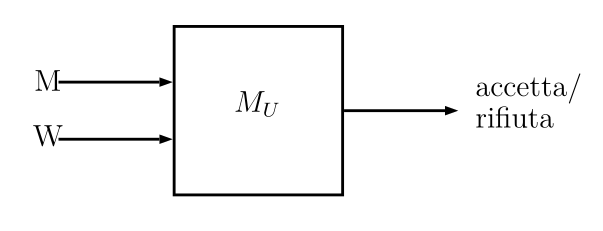
\includegraphics{2025-01-16_15-22.png}

	% \begin{center}
	% 	\psscalebox{1.0 1.0} % Change this value to rescale the drawing.
	% 	{
	% 		\begin{pspicture}(0,-1.2)(7.44,1.2)
	% 			\psframe[linecolor=black, linewidth=0.04, dimen=outer](4.36,1.2)(1.96,-1.2)
	% 			\psline[linecolor=black, linewidth=0.04, arrowsize=0.05291667cm 2.0,arrowlength=1.4,arrowinset=0.0]{->}(0.36,0.4)(1.96,0.4)
	% 			\psline[linecolor=black, linewidth=0.04, arrowsize=0.05291667cm 2.0,arrowlength=1.4,arrowinset=0.0]{->}(0.36,-0.4)(1.96,-0.4)
	% 			\psline[linecolor=black, linewidth=0.04, arrowsize=0.05291667cm 2.0,arrowlength=1.4,arrowinset=0.0]{->}(4.36,0.0)(5.96,0.0)
	% 			\rput[bl](0.02,0.28){M}
	% 			\rput[bl](0.0,-0.5){W}
	% 			\rput[bl](2.82,-0.08){$M_U$}
	% 			\rput[bl](6.2,0.1){accetta/}
	% 			\rput[bl](6.2,-0.24){rifiuta}
	% 		\end{pspicture}
	% 	}
	% \end{center}
	$$L_U\{(M,W)|W\in L(M)\}$$
	La macchina universale corrisponde alla nostra idea di computer programmabile. Descriviamo
	questa macchina universale, che ha quattro nastri:
	\begin{itemize}
		\item \textbf{primo nastro:} $M111W$
		\item \textbf{secondo nastro:} nastro/codifica di M
		\item \textbf{terzo nastro:} stato/codifica di M
		\item \textbf{quarto nastro:} ausiliario

	\end{itemize}
	Il linguaggio universale è ricorsivamente enumerabile ma non ricorsivo (non potrebbe esserlo, visto
	che la macchina che simula potrebbe non fermarsi).
	Il diagramma delle classi dei linguaggi è quindi diventato il seguente:
			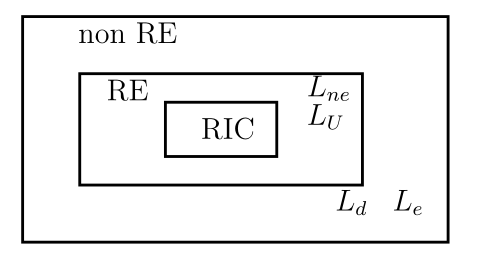
\includegraphics{2025-01-16_15-23.png}
	% \begin{center}
	% 	\psscalebox{1.0 1.0} % Change this value to rescale the drawing.
	% 	{
	% 		\begin{pspicture}(0,-1.6)(6.0,1.6)
	% 			\psframe[linecolor=black, linewidth=0.04, dimen=outer](6.0,1.6)(0.0,-1.6)
	% 			\psframe[linecolor=black, linewidth=0.04, dimen=outer](4.8,0.8)(0.8,-0.8)
	% 			\psframe[linecolor=black, linewidth=0.04, dimen=outer](3.6,0.4)(2.0,-0.4)
	% 			\rput[bl](0.8,1.2){non RE}
	% 			\rput[bl](1.2,0.4){RE}
	% 			\rput[bl](2.52,-0.14){RIC}
	% 			\rput[bl](4.0,0.4){$L_{ne}$}
	% 			\rput[bl](4.0,0.0){$L_U$}
	% 			\rput[bl](5.2,-1.2){$L_e$}
	% 			\rput[bl](4.4,-1.2){$L_d$}
	% 		\end{pspicture}
	% 	}
	% \end{center}
	Valgono ancora le riduzioni. Sapendo che $P_1$ è indecidibile (non RE o RE), posso fare una riduzione
	dalle istanze di $P_1$  alle istanze di $P_2$ mostrando che $P_2$ è indecidibile.
	Con la riduzione stiamo dicendo che $P_2$ è almeno difficile quanto $P_1$  (e non viceversa!).
	Notiamo che non è nemmeno necessario che tutte le istanze di $P_2$  siano "coperte" dal processo di
riduzione.
\begin{theorem}
	$$L_{ne}\in RE$$
\end{theorem}
\begin{proof}
	Dobbiamo fare una riduzione da $L_u$ a $L_{ne}$ per mostrare che $L_{ne}$ è ricorsivamente enumerabile.
	La riduzione è descritta da questo schema:
	\begin{center}
			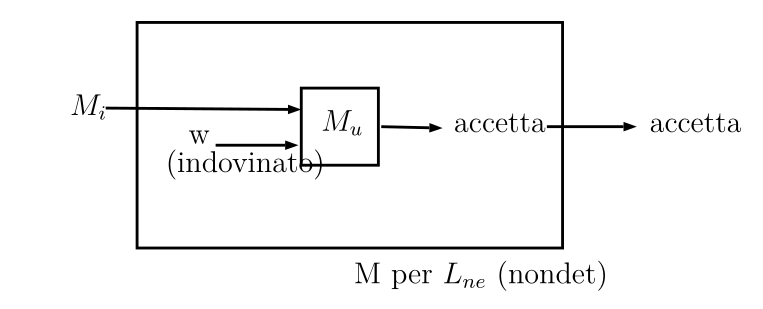
\includegraphics{2025-01-16_15-25.png}
		% \psscalebox{1.0 1.0} % Change this value to rescale the drawing.
		% {
		% 	\begin{pspicture}(0,-1.89)(9.2,1.89)
		% 		\psframe[linecolor=black, linewidth=0.04, dimen=outer](6.92,1.89)(0.92,-1.31)
		% 		\psframe[linecolor=black, linewidth=0.04, dimen=outer](4.34,0.97)(3.22,-0.15)
		% 		\psline[linecolor=black, linewidth=0.04, arrowsize=0.05291667cm 2.0,arrowlength=1.4,arrowinset=0.0]{->}(0.5,0.67)(3.24,0.65)
		% 		\psline[linecolor=black, linewidth=0.04, arrowsize=0.05291667cm 2.0,arrowlength=1.4,arrowinset=0.0]{->}(2.04,0.15)(3.2,0.15)
		% 		\psline[linecolor=black, linewidth=0.04, arrowsize=0.05291667cm 2.0,arrowlength=1.4,arrowinset=0.0]{->}(4.36,0.41)(5.22,0.39)
		% 		\psline[linecolor=black, linewidth=0.04, arrowsize=0.05291667cm 2.0,arrowlength=1.4,arrowinset=0.0]{->}(6.68,0.41)(7.94,0.41)
		% 		\rput[bl](5.38,0.33){accetta}
		% 		\rput[bl](8.12,0.33){accetta}
		% 		\rput[bl](1.66,0.17){w}
		% 		\rput[bl](1.34,-0.33){(indovinato)}
		% 		\rput[bl](0.0,0.51){$M_i$}
		% 		\rput[bl](3.52,0.29){$M_u$}
		% 		\rput[bl](3.98,-1.89){M per $L_{ne}$ (nondet)}
		% 	\end{pspicture}
		% }
	\end{center}
\end{proof}
\begin{theorem}
	$$L_{ne}\not\in RIC$$
\end{theorem}
\begin{proof}
	infatti essendo $l_e$ il complementare di $l_{ne}$, per i teoremi visti in precedenza  $l_e$ non può essere ricorsivo
	né può essere ricorsivamente enumerabile. Segue che  $l_e$ è non RE
\end{proof}
\begin{example}
	considero:
	$$L_e=\{M|\,L(M)=\emptyset\}$$
	$$L_{ne}=\{M|\,L(M)=\emptyset\}$$
\end{example}
%%% Local Variables:
%%% mode: LaTeX
%%% TeX-master: ../libro-linguaggi
%%% End:
